\documentclass[12pt]{report}

\setlength\parindent{0cm}

%------------------- declaring packages---------------------------------


% styling and graphics-based

\usepackage{graphicx} 
\usepackage{emptypage}
\usepackage[a4paper,
left=3cm,
right=3cm,
top=3cm,
bottom=3cm]{geometry}
\usepackage[percent]{overpic}
\usepackage{setspace}
\usepackage{pgf}
\usepackage{pgffor}
\usepackage{svg}
\usepackage{xcoffins}
\usepackage{xcolor}
\usepackage{caption}
\usepackage{changepage}
\usepackage{fontspec}
\setmainfont{Arial}

\doublespacing

%define colors
% Define custom colors
\definecolor{blueBase}{RGB}{70,130,180}
\definecolor{linkblue}{RGB}{0, 102, 204}
\definecolor{blueLeaf}{RGB}{135,206,250}

\definecolor{greenBase}{RGB}{34,139,34}
\definecolor{greenLeaf}{RGB}{144,238,144}

\definecolor{orangeBase}{RGB}{255,140,0}
\definecolor{orangeLeaf}{RGB}{255,200,120}

\definecolor{purpleBase}{RGB}{138,43,226}
\definecolor{purpleLeaf}{RGB}{186,85,211}

\definecolor{redBase}{RGB}{178,34,34}
\definecolor{redLeaf}{RGB}{240,128,128}

\definecolor{grayBase}{RGB}{105,105,105}
\definecolor{grayLeaf}{RGB}{169,169,169}

\definecolor{lightblue}{RGB}{225,245,254}
\definecolor{highlightblue}{RGB}{144,202,249}

\definecolor{lightgray}{RGB}{240,240,240}
\definecolor{highlightgray}{RGB}{200,200,200}

\definecolor{darkgreenMW}{RGB}{0, 170, 0} % or choose your own color
\definecolor{lightgreenMW}{RGB}{144,238,144}

% for figures and tables

% figures:
\usepackage{subcaption}
\renewcommand{\thesubfigure}{\Alph{subfigure}}
\usepackage{forloop}
\newcounter{subfigurenumber}
\newcommand{\subplot}[5]{%
  \begin{subfigure}[t]{1\textwidth}
    \centering
    \includegraphics[#2]{#3}
    \phantomcaption\label{sub0:#5}
  \end{subfigure}
  \forloop{subfigurenumber}{1}{\value{subfigurenumber} < #1}{%
    \parbox{0pt}{\phantomsubcaption\label{sub\arabic{subfigurenumber}:#5}}
  }
  \vspace{-0.8cm}
  \caption{#4}\label{#5}
}
% Define subplot with overpic and manual label positioning
\newcounter{customsubfig}
\newcommand{\customsubplot}[8]{%
  \begin{subfigure}[t]{1\textwidth}
    \centering
    \begin{overpic}[width=#2, trim=#3, clip]{#4}
        \put(#5){\large\text{(A)}}
        \put(#6){\large\text{(B)}}
        \phantomcaption\label{sub0:#7}%
    \end{overpic}
\end{subfigure}
\forloop{customsubfig}{1}{\value{customsubfig} < #1}{%
    \parbox{0pt}{\phantomsubcaption\label{sub\arabic{customsubfig}:#7}}
  }
    \vspace{-0.8cm}  
    \caption{#8}
    \label{#7}
}
\usepackage[export]{adjustbox}
\usepackage{wrapfig}
\usepackage{rotating}
\usepackage{lscape}
\usepackage{tikz}
\usetikzlibrary{arrows.meta, positioning, shapes.geometric, 3d, calc}
\usepackage{pgfmath-xfp}
\usepackage{tikz-3dplot}
\tikzset{plane/.style n args={3}{insert path={%
#1 -- ++ #2 -- ++ #3 -- ++ ($-1*#2$) -- cycle}},
unit xy plane/.style={plane={#1}{(1,0,0)}{(0,1,0)}},
unit xz plane/.style={plane={#1}{(1,0,0)}{(0,0,1)}},
unit yz plane/.style={plane={#1}{(0,1,0)}{(0,0,1)}},
get projections/.style={insert path={%
let \p1=(1,0,0),\p2=(0,1,0)  in 
[/utils/exec={\pgfmathtruncatemacro{\xproj}{sign(\x1)}\xdef\xproj{\xproj}
\pgfmathtruncatemacro{\yproj}{sign(\x2)}\xdef\yproj{\yproj}
\pgfmathtruncatemacro{\zproj}{sign(cos(\tdplotmaintheta))}\xdef\zproj{\zproj}}]}},
pics/unit cube/.style={code={\path[get projections];
\draw (0,0,0) -- (1,1,1);
\ifnum\zproj=-1
 \path[3d cube/every face,3d cube/xy face,unit xy plane={(0,0,0)}]; 
\fi
\ifnum\yproj=1
 \path[3d cube/every face,3d cube/yz face,unit yz plane={(1,0,0)}]; 
\else
 \path[3d cube/every face,3d cube/yz face,unit yz plane={(0,0,0)}]; 
\fi
\ifnum\xproj=1
 \path[3d cube/every face,3d cube/xz face,unit xz plane={(0,0,0)}]; 
\else
 \path[3d cube/every face,3d cube/xz face,unit xz plane={(0,1,0)}]; 
\fi
\ifnum\zproj>-1
 \path[3d cube/every face,3d cube/xy face,unit xy plane={(0,0,1)}]; 
\fi
}},
3d cube/.cd,
xy face/.style={fill=blue!10},
xz face/.style={fill=blue!20},
yz face/.style={fill=blue!30},
num cubes x/.estore in=\NumCubesX,
num cubes y/.estore in=\NumCubesY,
num cubes z/.estore in=\NumCubesZ,
num cubes x=1,num cubes y/.initial=1,num cubes z/.initial=1,
cube scale/.initial=0.9,
every face/.style={draw,very thick},
/tikz/pics/.cd,
cube array/.style={code={%
 \tikzset{3d cube/.cd,#1}
 %\typeout{\NumCubesX,\NumCubesY,\NumCubesZ}
  \path[get projections];
  \ifnum\yproj=1
   \def\LstX{1,...,\NumCubesX}
  \else 
   \ifnum\NumCubesX>1
    \pgfmathtruncatemacro{\NextToLast}{\NumCubesX-1}
    \def\LstX{\NumCubesX,\NextToLast,...,1}
   \else
    \def\LstX{1}   
   \fi 
  \fi
  \ifnum\xproj=-1
   \def\LstY{1,...,\NumCubesY}
  \else 
   \ifnum\NumCubesY>1
    \pgfmathtruncatemacro{\NextToLast}{\NumCubesX-1}
    \def\LstY{\NumCubesY,\NextToLast,...,1}
   \else
    \def\LstY{1}   
   \fi 
  \fi
  \ifnum\zproj=1
   \def\LstZ{1,...,\NumCubesZ}
  \else 
   \ifnum\NumCubesZ>1
    \pgfmathtruncatemacro{\NextToLast}{\NumCubesX-1}
    \def\LstZ{\NumCubesZ,\NextToLast,...,1}
   \else
    \def\LstZ{1}   
   \fi 
   \def\LstZ{\NumCubesZ,\NextToLast,...,1}
  \fi
  \foreach \X in \LstX
  {\foreach \Y in \LstY
   {\foreach \Z in \LstZ
    {\ifnum\X=4
      \ifnum\Y=2
        \path (\X-\NumCubesX/2-1,\Y-\NumCubesY/2-1,\Z-\NumCubesZ/2-1)
          pic[scale=\pgfkeysvalueof{/tikz/3d cube/cube scale},
               3d cube/.cd,
               xy face/.style={fill=red!10},
               xz face/.style={fill=red!20},
               yz face/.style={fill=red!30}]{unit cube};
      \else
        \path (\X-\NumCubesX/2-1,\Y-\NumCubesY/2-1,\Z-\NumCubesZ/2-1)
          pic[scale=\pgfkeysvalueof{/tikz/3d cube/cube scale}]{unit cube};
      \fi
    \else
      \path (\X-\NumCubesX/2-1,\Y-\NumCubesY/2-1,\Z-\NumCubesZ/2-1)
        pic[scale=\pgfkeysvalueof{/tikz/3d cube/cube scale}]{unit cube};
    \fi
  }}
  } 
}}
}
% tables:
\usepackage{tabularx,ragged2e,booktabs,caption}
\usepackage{multicol,tabularx,capt-of}
\usepackage{hhline}
\usepackage{multirow}
\usepackage{array}
\usepackage[edges]{forest}


% for math equations

\usepackage{amssymb}
\usepackage{float}
\usepackage{verbatim}
\usepackage{amsmath} 
\usepackage{amsthm}   


% for acronyms and glossaries

\usepackage{acronym}
\usepackage{glossaries}
\usepackage{placeins}

% for hyperlinks

\usepackage[round]{natbib}

\usepackage[colorlinks = true,
            linkcolor = black,
            urlcolor  = linkblue,
            citecolor = black,
            anchorcolor = black]{hyperref}
\newcommand{\figref}[1]{\hyperref[#1]{(Fig.~\ref*{#1})}}
\newcommand{\tabref}[1]{\hyperref[#1]{(Tab.~\ref*{#1})}}
\usepackage{url}
\def\UrlBreaks{\do\/\do-}

\usepackage[normalem]{ulem}  % for underline

\usepackage{cleveref}

\usepackage{sectsty}
\allsectionsfont{\bfseries}
\chapterfont{\centering\Large}
\sectionfont{\normalsize}
\subsectionfont{\normalsize}


\usepackage [english]{babel}
\usepackage [autostyle, english = british]{csquotes}
\MakeOuterQuote{"}

%url
% header formatting

\usepackage{layout}
\usepackage{fancyhdr}

\fancypagestyle{custompagestyle}{%
    \fancyhf{}
    \fancyfoot[R]{\thepage}
}

\fancypagestyle{noheaderfooter}{%
    \fancyhf{} % Clear header and footer
    \renewcommand{\headrulewidth}{0pt} % Remove header line
}
\usepackage{titlesec}  % Import titlesec for custom chapter formatting

% Remove "Chapter" and display number inline with title
\renewcommand{\thechapter}{\arabic{chapter}}  % Only display chapter number
\titleformat{\chapter}[hang]{\normalfont\Huge\bfseries\centering}
{\thechapter}{1em}{}

\titlespacing*{\chapter}{0pt}{-50pt}{20pt} 

%appendix formatting
\usepackage{appendix}
\usepackage{microtype}

%footer formatting

\interfootnotelinepenalty=10000

\def\cx{.85} % relative size of cube vs grid unit
\newcommand{\cube}[4][black]{
  \fill[#1!20] (#2,#3,#4) -- (#2+\cx,#3,#4) -- (#2+\cx,#3+\cx,#4) -- (#2,#3+\cx,#4) -- cycle;
  \fill[#1!10] (#2,#3+\cx,#4) -- (#2,#3+\cx,#4-\cx) -- (#2+\cx,#3+\cx,#4-\cx) -- (#2+\cx,#3+\cx,#4) -- cycle;
  \fill[#1!30] (#2+\cx,#3,#4) -- (#2+\cx,#3+\cx,#4) -- (#2+\cx,#3+\cx,#4-\cx) -- (#2+\cx,#3,#4-\cx) -- cycle;
}

% specify files to use, especially useful if you want to build only one chapter due to build time
%\includeonly{introduction}

%----------------------------begin document-------------------------------
\setcounter{secnumdepth}{2}  % Chapters and sections are numbered
\counterwithout{figure}{chapter}
\counterwithout{table}{chapter}
\counterwithout{equation}{chapter}

\sloppy

\begin{document}

%\frontmatter
\pagenumbering{gobble}

\begin{titlepage}
    \begin{center}
        
% Insert logos (left center and right)


\begin{minipage}{0.3\textwidth}
    \begin{flushleft}
        
\includegraphics[height=1.8cm]{Figures/logo_cob.png} % Replace with your left logo
    \end{flushleft}
  \end{minipage}
  \hfill
  \begin{minipage}{0.3\textwidth}
    \begin{center}
      
\includegraphics[height=2cm]{Figures/logo_imbrsea.png} % Replace with your center logo
    \end{center}
  \end{minipage}
  \hfill  
  \begin{minipage}{0.3\textwidth}
    \begin{flushright}
      
\includegraphics[height=3cm]{Figures/logo_ghent.png} % Replace with your right logo
    \end{flushright}
  \end{minipage}
  
  \vspace{1.8cm}
  
  % Title of the Thesis
  \begin{center}
    {\LARGE \textbf{Spatio-temporal fishing risk of large pelagic fish in the Mediterranean Sea}}\\[0.5cm]
  
    \textbf{Master Thesis}\\[0.5cm]
    of\\[0.5cm]
    \textbf{Tom Leven}\\[0.5cm]
    02312706\\[1.5cm]
  
    % Department and Institute information
    At the Faculty of Sciences\\
    Ghent University\\[1.5cm]
  
    Main supervisor: Dr. Pilar Tugores\\
    Co-supervisors: Dr. Diego Alvarez-Berastegui \& Dr. Miguel Cabanellas-Reboredo


    \end{center}
  \end{center}

\end{titlepage}


% Start Roman numbering AFTER the disclaimer
\newpage
\pagenumbering{roman}

\chapter*{Executive Summary}

The executive summary goes here.

\addcontentsline{toc}{chapter}{Executive Summary}

\chapter*{Abstract}

Abstract goes here.

\addcontentsline{toc}{chapter}{Abstract}

\tableofcontents{}

%\listoftables{}

%\listoffigures{}

\thispagestyle{noheaderfooter}
\cleardoublepage

\pagenumbering{arabic}
\setcounter{page}{1}

\chapter{Introduction}


Fish are great.

\section{Overview of tools}

Lorem ipsum dolor sit amet \citep{paolo24satellite}.

\section{Friends}

\chapter{Material and Methods}

Lorem ipsum dolor sit amet \cite{paolo24satellite}.

\section{Data analysis}

\chapter{Results}
\section{Cumulative apparent fishing hours}
A total of 213 unique longliners and purse seiners were recorded for 2015-2024. These vessels
together accounted for an average of 122 760 hours per year, with an average of 576 hours per
vessel per year. Areas that show the highest effort throughout the study time include the
Mediterranean coast of Spain, around Sardinia and Sicily, south of Malta, the Adriatic, and south
of Cyprus \figref{sub0:fig:sum_cv}. Areas with high effort generally also show the lowest
coefficient of variation \figref{sub1:fig:sum_cv}. There does not appear to be any fishing activity
based on AIS around the African Mediterranean coast \figref{fig:sum_cv}.

\medskip

\begin{figure}[ht]
	\subplot{2}
	{width=1\linewidth, trim=1.2cm 0 1.2cm 0,clip}
	{Figures/plots/sum_cv.pdf}
	{%
		Summary statistics for both longliners and purse-seiners. \subref{sub0:fig:sum_cv}) Cumulative fishing hours in the Mediterranean (2015-2024).
		Colors are on a log-scale. \subref{sub1:fig:sum_cv}) Coefficient of variation between years (standard deviation divided by mean) for each cell.
	}{fig:sum_cv}
\end{figure}

\FloatBarrier
\section{Fishing hotspots and high risk areas}
Numerous persistent longline hotspot areas were identified throughout the Mediterranean including
the southern coast of Spain, south of Sardinia, around Sicily and Malta, as well as south of Cyprus
\figref{sub0:fig:longline_hotspots}. These hotspots show however, differing trends. Fishing hours
in the south of Malta appear to be increasing throughout, with a similar trend of increase in the
Adriatic Sea. Other areas that appear to be consistent hotspots, like the east of Sicily, show a
decreasing trend \figref{sub1:fig:longline_hotspots}.

\begin{figure}[H]
	\subplot{2}
	{width=1\linewidth, trim=0.85cm 0 1.2cm 0,clip}
	{Figures/plots/dll_hotspot_trend.pdf}
	{%
		Hotspot percentage and trend scores for longliners in the Mediterranean.
		The percentage reflects the years in which a given cell was a hotspot based on the Getis-Ord Gi* statistic.
		The Z-score is derived from the Mann-Kendall statistic.}
	{fig:longline_hotspots}
\end{figure}

Purse seine hotspots appear persistent around the Balearic Islands, in the Adriatic Sea, and along
the Calabrian coast in Italy \figref{sub0:fig:seines_hotspots}. Trends in these areas show a clear
increase around Ibiza and in the central Adriatic, while areas around the coast in the Adriatic
show a decrease \figref{sub1:fig:seines_hotspots}. The hotspot area along Calabria shows no clear
trend.

\begin{figure}[ht]
	\subplot{2}
	{width=1\linewidth, trim=0.4cm 0 0.7cm 0,clip}
	{Figures/plots/pss_hotspot_trend.pdf}
	{%
		Hotspot percentage and trend scores for purse seiners in the Mediterranean.
		The percentage reflects the years in which a given cell was a hotspot based on the Getis-Ord Gi* statistic.
		The Z-score is derived from the Mann-Kendall statistic.}
	{fig:seines_hotspots}
\end{figure}

\FloatBarrier
\section{Temporal changes}
Longline fishing hours show a clear seasonal trend where activity is highest during warmer months
(mainly in the summer) and lowest in the colder months around winter
\figref{sub0:fig:longlines_ridge}. Some areas show high effort earlier in the season in spring (for
example south of Malta) and others are more persistent later in the season in fall (for instance
around Ibiza). The time series show a similar seasonal trend, although the intensity varies between
years, and it appears that the longline season is expanding between years
\figref{sub1:fig:longlines_ridge}. The highest annual longline fishing hours throughout the study
time were recorded for 2022 and the lowest for 2015 \tabref{tab:year_hours}.

\begin{figure}[H]
	\customsubplot{2}
	{1\linewidth}                           % width
	{0.5cm 0 0.6cm 0}                       % trim
	{Figures/plots/longlines_ridge_seasons.pdf} % file
	{5,92}                                  % (A) position
	{5,40}                                  % (B) position
	{fig:longlines_ridge}
	{%
		Temporal changes in longline fishing hours. \subref{sub0:fig:longlines_ridge}) Spatial differences between seasons.
		Hours are summed per season and cell and colour is on a log-scale. Seasons are defined based on calendar dates:
		winter (Dec 21 - Mar 19), spring (Mar 20 - Jun 20), summer (Jun 21 - Sep 21), and fall (Sep 22 - Dec 20). \subref{sub1:fig:longlines_ridge})
		Time series of fishing hours, summed per year and day.}
\end{figure}

\begin{table}[ht]
	\centering
	\caption{Annual sum of fishing hours for purse seiners and longliners.}
	\medskip
	\begin{tabular}{lcc}
		\toprule
		\textbf{Year} & \multicolumn{2}{c}{\textbf{Fishing hours}}                       \\
		\cmidrule(lr){2-3}
		              & \textbf{Purse seiners}                     & \textbf{Longliners} \\
		\midrule
		2015          & 4,193                                      & 71,846              \\
		2016          & 5,313                                      & 89,136              \\
		2017          & 5,901                                      & 107,345             \\
		2018          & 6,128                                      & 106,130             \\
		2019          & 5,931                                      & 113,261             \\
		2020          & 5,636                                      & 124,927             \\
		2021          & 5,706                                      & 133,361             \\
		2022          & 5,675                                      & 149,059             \\
		2023          & 5,085                                      & 139,068             \\
		2024          & 6,661                                      & 137,406             \\
		\bottomrule
	\end{tabular}
	\label{tab:year_hours}
\end{table}

Regarding the purse seine fleet, fishing hours show a very pronounced seasonal trend with a peak in
spring \figref{fig:seines_ridge}. The core areas of the fishery during spring are the Balearic
Islands, along the coast of Calabria (south-west Italy), and the central Adriatic. In the Adriatic,
there appears to be purse seine activity throughout the whole year \figref{sub0:fig:seines_ridge}.
The purse seine season for large-pelagic species is limited to the months of May and June and is
consistent between years \figref{sub1:fig:seines_ridge}. Highest annual fishing hours for purse
seiners were recorded in 2024 and the lowest in 2015 \tabref{tab:year_hours}.

\begin{figure}[ht]
	\customsubplot{2}
	{1\linewidth}
	{1.2cm 0 0.9cm 0}                       % trim
	{Figures/plots/purse_seines_ridge_seasons.pdf} % file
	{3,93.5}                                  % (A) position
	{3,42}                                  % (B) position
	{fig:seines_ridge}
	{%
		Temporal changes in purse seine fishing hours. \subref{sub0:fig:seines_ridge}) Spatial differences between seasons. Seasons are defined based on calendar dates:
		winter (Dec 21 - Mar 19), spring (Mar 20 - Jun 20), summer (Jun 21 - Sep 21), and fall (Sep 22 - Dec 20).
		Hours are summed per season and cell and colour is on a log-scale. \subref{sub1:fig:seines_ridge}) Time series of fishing hours, summed per year
		and day.}
\end{figure}

\FloatBarrier
\section{Flag countries}

Vessels were flagged to a total of 10 countries and the majority of vessels analysed were
longliners (Tab.~\ref{tab:countries_vessels}; see Fig.~\ref{fig:longline_effort_countries}
and~\ref{fig:seine_effort_countries} for a spatial overview by country). Italy shows the highest
amount of both purse seiners and longliners identified in the GFW data.

\medskip

\begin{table}[ht]
	\centering
	\caption{Number of vessels by country and gear type in 2024 from our detections compared to vessels with drifting longlines currently registered with the GFCM and
		tuna purse seine vessels currently registered with ICCAT (June, 2025). ‘--’ indicates no recorded vessels for that gear. PS = purse seiners, LL = longliners}
	\medskip
	\begin{tabularx}{\textwidth}{l *{6}{>{\centering\arraybackslash}X}}
		\toprule
		\textbf{Country}      & \textbf{Detected PS} & \textbf{Reg. PS} & \textbf{\% PS}  & \textbf{Detected LL} & \textbf{Reg. LL} & \textbf{\% LL}  \\
		\midrule
		Albania               & --                   & 2                & 0.0\%           & --                   & --               & --              \\
		Algeria               & 3                    & 39               & 7.7\%           & --                   & --               & --              \\
		EU-Croatia            & 2                    & 3                & 66.7\%          & --                   & --               & --              \\
		EU-Cyprus             & --                   & 1                & 0.0\%           & 14                   & 15               & 93.3\%          \\
		Egypt                 & --                   & 2                & 0.0\%           & --                   & --               & --              \\
		EU-France             & 13                   & 21               & 61.9\%          & --                   & 4                & 0.0\%           \\
		EU-Greece             & --                   & --               & --              & 8                    & 24               & 33.3\%          \\
		EU-Italy              & 16                   & 19               & 84.2\%          & 60                   & 83               & 72.3\%          \\
		EU-Malta              & --                   & 2                & 0.0\%           & 19                   & 17               & 111.8\%         \\
		Libya                 & --                   & 15               & 0.0\%           & --                   & --               & --              \\
		Morocco               & 1                    & 5                & 20.0\%          & --                   & --               & --              \\
		EU-Spain              & 5                    & 7                & 71.4\%          & 22                   & 30               & 73.3\%          \\
		Tunisia               & --                   & 59               & 0.0\%           & --                   & --               & --              \\
		Turkey                & --                   & 36               & 0.0\%           & --                   & --               & --              \\
		\midrule
		\textbf{Total / Mean} & \textbf{40}          & \textbf{213}     & \textbf{30.1\%} & \textbf{123}         & \textbf{173}     & \textbf{58.6\%} \\
		\bottomrule
	\end{tabularx}
	\label{tab:countries_vessels}
\end{table}

Most regions with high fishing activity are fishing grounds shared by multiple countries
\figref{fig:no_countries}. Regions with high overlap between flag countries for longliners include
the Balearic Islands, south of Crete, and south of Malta, which are also areas with high fishing
hours \figref{sub0:fig:sum_cv}. For purse seiners, fishing generally is more concentrated and thus,
overlap is also higher, as seen in the core fishing areas of the Balearic Islands and south of
Malta \figref{fig:no_countries}.

\begin{figure}[H]
	\centering
	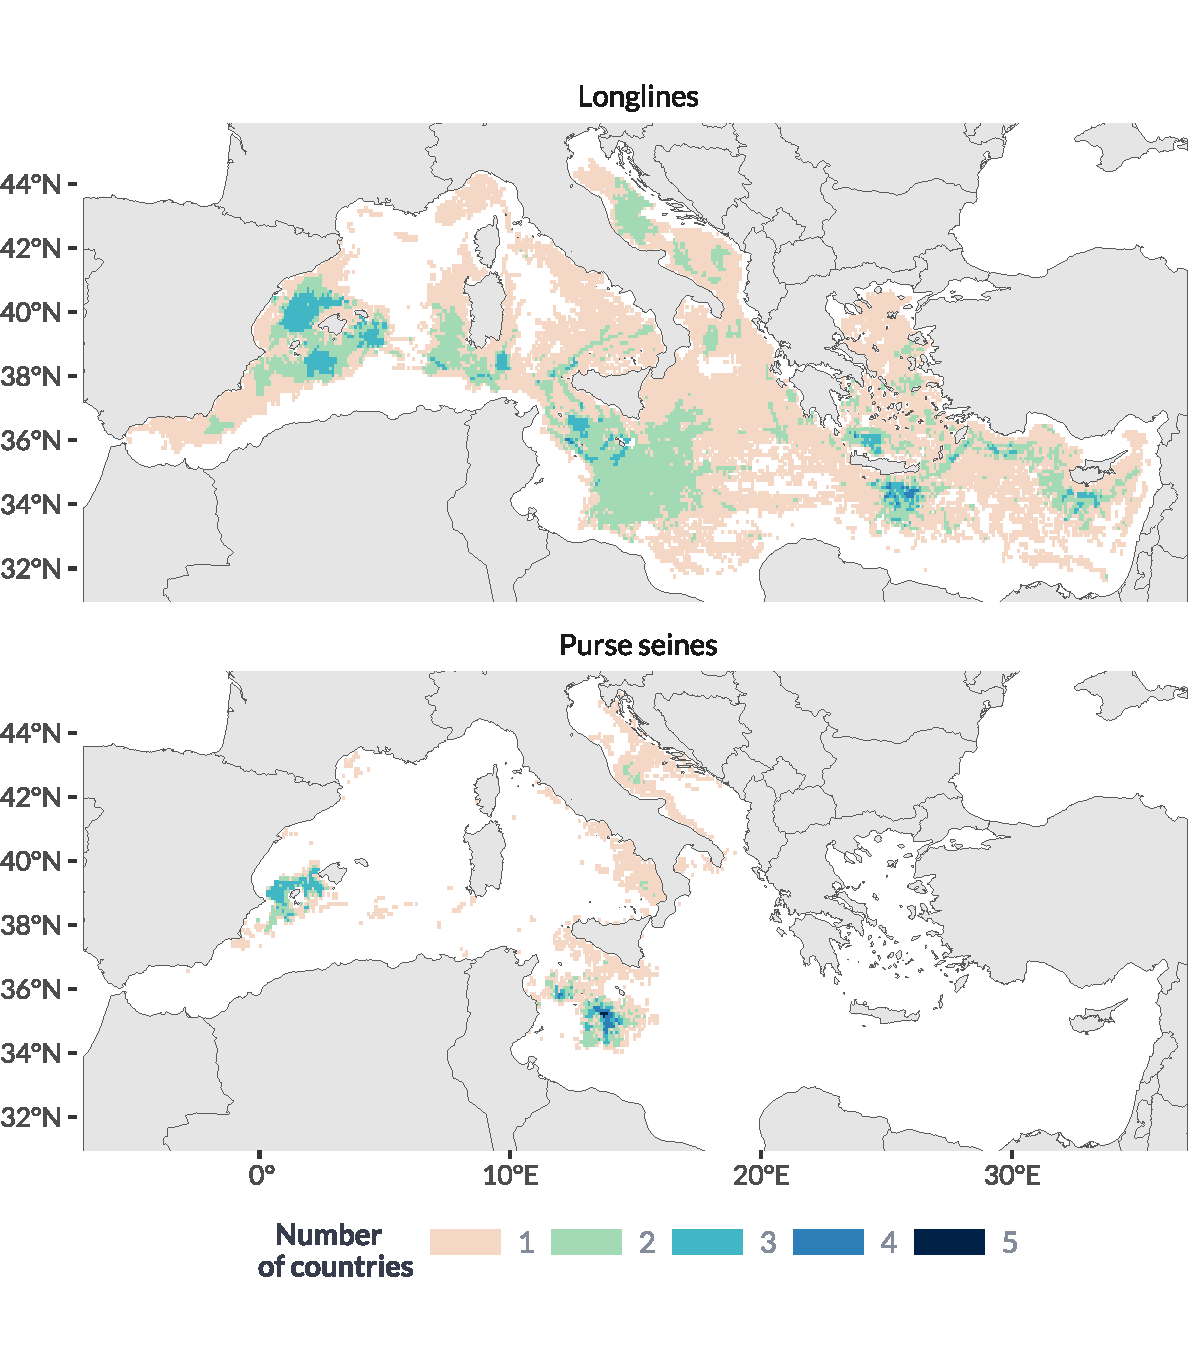
\includegraphics[width=1\linewidth, trim=0 1.2cm 0 1.2cm,clip]{Figures/plots/no_countries.pdf}
	\caption{Number of countries fishing per cell for longliners and purse seiners between 2015-2024.}
	\label{fig:no_countries}
\end{figure}

A comparison of fishing hours from the GFW data with catch data from ICCAT shows that AIS
under-represents fishing activity by non-EU countries relative to EU countries
\figref{fig:ais_iccat}. Even though, many non-EU countries account for a substantial share of the
total reported catches. Notably, AIS also does not capture any French longline vessels.

\begin{figure}[ht]
	\centering
	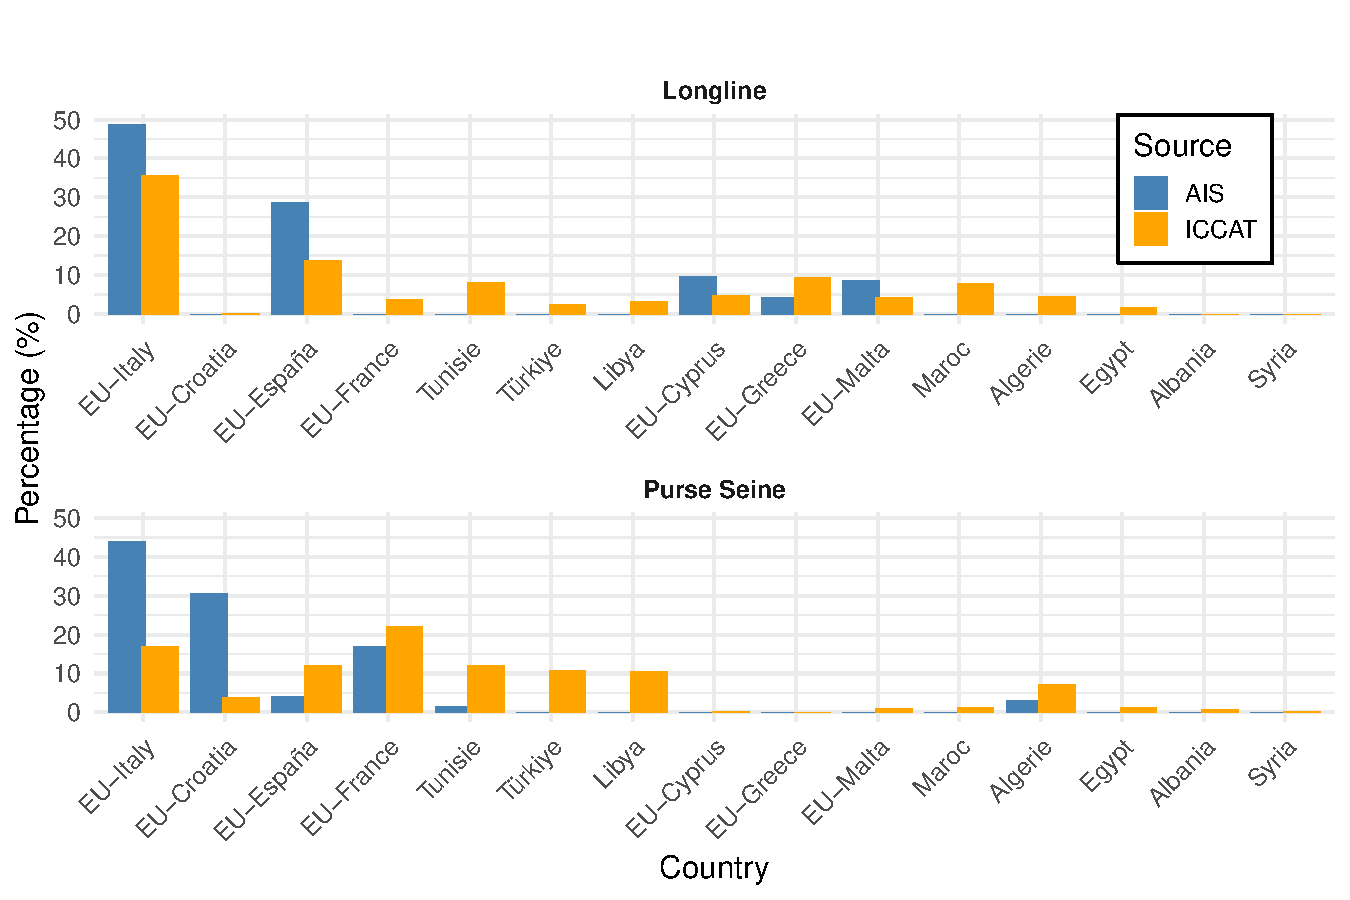
\includegraphics[width=1\linewidth, trim=0 0 0 1cm,clip]{Figures/plots/ais_vs_iccat.pdf}
	\caption{Comparison of relative percentages between GFW AIS data and ICCAT catch data. AIS percentages are relative to the
		total fishing hours between all countries. ICCAT percentages are relative to the total weight of catches between all countries.}
	\label{fig:ais_iccat}
\end{figure}

\FloatBarrier
\section{Depth and distance to port}

The relationship between the cumulative proportion of fishing hours and the distance to port
reveals that most fishing activity of both gear types is concentrated less than 100 km from the
closest port \figref{sub0:fig:depth_dist}. The trend for the depth is different between gear types,
where most purse seine fishing occurs at shallower depths (> 1000 m; 50\% above 500 m depth) and
longline fishing takes place over much greater depth ranges (Fig.~\ref{sub1:fig:depth_dist}; 50\%
above 1600 m depth).

\begin{figure}[ht]
	\customsubplot{2}
	{1\linewidth}                           % width
	{0 0 0 0}                       % trim
	{Figures/plots/depth_dist_both.pdf} % file
	{12,67}                                  % (A) position
	{58,67}                                  % (B) position
	{fig:depth_dist}
	{%
		Cumulative proportion of fishing hours with \subref{sub0:fig:depth_dist}) Distance to port and \subref{sub1:fig:depth_dist}) Depth.}
\end{figure}


\chapter{Discussion}
In this study, the fishing activity targetting large pelagic fishes (LPF) across the Mediterranean
Sea was analysed. Strong spatial and temporal patterns in how fishing is distributed, as well as
regional hotspots were identified. Furthermore, the utility of AIS in monitoring industrial LPF
fleets was shown, while a big gap in the uptake of AIS technology between countries in southern and
northern Mediterranean countries was found.

\section{Main risk areas (hotspots)}
Fishing hotspots and thus, the main risk areas for LPF, aligned with the species' known aggregation
sites, particularly around the Balearic Islands, the Tyrrhenian Sea, the Adriatic Sea, and off the
coasts of Cyprus and Malta. These hotspot regions overlap with key spawning and feeding areas
identified in previous studies \citep{medina_spawning,arocha_2007}. A prime example of this is the
migration of large (>150 kg) bluefin tuna (BFT) from the Atlantic towards their spawning regions in
the Mediterranean between mid-May until mid-July, which drives intense seasonal purse seine
activity \citep{bft_mig_med}. However, some smaller individuals remain resident in the
Mediterranean the whole year-round \citep{cermeno_15_tagging,heinisch_08}. The presence of this
all-year-round stock might explain the extended season of longliners. The spatio-temporal
distribution of the purse seiners around the Balearic Islands, and the Tyrrhenian Sea indicates
that they target known spawning grounds \citep{medina_spawning}. Interestingly, the spawning area
around the Strait of Sicily was not consistently identified as a purse seine hotspot even though
this area is frequented by fleets of up to 5 countries. This is likely because of a lack in the
adoption of AIS by non-EU countries, which is one potential handicap of AIS derived fishing
activity \citep{taconet2019global,paolo24satellite}.

\medskip

The Adriatic Sea appeared to be the most consistent purse seine hotspot identified in our study and
is frequented by purse seiners from Italy and Croatia (Fig.~\ref{fig:seines_hotspots}
and~\ref{fig:seine_effort_countries}). Contrary to the narrow temporal window of the purse seine
activity in the rest of the Mediterranean (which follows the spawning aggregations and the allowed
fishing season) the Adriatic fleet operates in all seasons, particularly vessels flagged to Croatia
(Fig.~\ref{fig:seines_ridge} and~\ref{fig:seine_effort_countries}). This might not only be
explained by ecological aspects like the presence of smaller individuals throughout the whole year,
but also due to socio-economic aspects and the fact that Croatia and Italy are the only countries
permitted to catch individuals < 30 kg for the use in tuna farms (Fig.~\ref{fig:hrv};
\citealp{hrv_farms}).

\medskip

The centroid of the purse seine hotspot around the Balearic Islands showed temporal variability and
moved from the north-west of Ibiza more towards the south and the Mallorca channel
\figref{fig:pss_yearly}. This could relate to the position of a frontal region which has been shown
to be spatially dynamic over time, and important for the spawning location of BFT
\citep{balbin_14,reglero_12}. Other species whose migratory patterns support the fishing activity
found here is swordfish (\textit{Xiphias gladius}). Swordfish in the Mediterranean Sea are
genetically distinct and only show limited migration between there and the Atlantic. Migratory
patterns are highly complex in general and poorly studied within the Mediterranean Sea. Spawning
migration is however linked to thermal fronts, particularly the 24\textdegree C isotherm
\citep{palko1981swordfish,arocha_2007}. Corresponding to this, they spawn from June to August in
areas west of the Balearic Islands until the Strait of Gibraltar, in the Tyrrhenian Sea and the
Strait of Messina, the Levantine Sea, and the Gulf of Taranto in the Ionian Sea (see Fig. 5 in
\citealp{arocha_2007}). They are targeted mainly by the longline fleet and corresponding hotspots
overlapped closely with these spawning areas, particularly in the western Mediterranean and the
Tyrrhenian region.

\medskip

Our analysis did not reveal clear temporal trends within most swordfish longline hotspots. This is
likely due to the use of different types of longlines targeting various species, which are all
analysed together in our study. As a result, we are limited in linking observed patterns within
each hotspot to the specific, dynamic habitat use of individual species, as we were able to do for
the purse seine fishery targeting bluefin tuna around the Balearic Islands.

\medskip

Monitoring the fine-scale spatio-temporal dynamics of the swordfish longline fishery is still
however, particularly valuable because juveniles and adults occupy distinct habitats: juveniles
tend to remain in coastal waters, while adults are more associated with deeper, pelagic zones
\citep{damalas_14_swo}. This spatial segregation by life stage offers an opportunity for more
targeted monitoring and management. AIS data can for example help identify when and where longline
fishing activity occurs close to shore, potentially indicating higher risks of juvenile bycatch.
Such information could be used to assess compliance with existing regulations, guide the
implementation of spatial or seasonal closures, and evaluate whether these are effectively
protecting juvenile habitats. Given that juvenile catch rates were still high prior to the 2017
introduction of a minimum size limit of 100 cm lower jaw fork length, and that discards have since
increased due to undersized individuals being caught, spatially explicit monitoring tools like AIS
could support more adaptive and precise management of the fishery
\citep{iccat_juvenile_catches_swo,iccat_juvenile_swo_ortiz,iccat_swo_discards}.

\medskip

Hotspots in general however, are quite consistent along our study period (2015-2024), and the main
fishing grounds stay the same (Fig.~\ref{fig:dll_yearly} and~\ref{fig:pss_yearly}). This might be
related to the large-scale stability of the spawning and feeding grounds of the LPF targeted. This
should however be closely monitored in the future considering the big impacts of climate change on
the Mediterranean Sea (REF). Tracking fisheries spatially and comparing data between different
years might provide early signs of changes in the distribution of these species, especially when
combined with logbook catch data (e.g., \citealp{campos_ais_logbook}). The clear seasonality of the
purse seine fleet can be attributed to the timing of BFT migration into the Mediterranean and the
implemented seasonal closures and TAC's decided upon by ICCAT, which are usually reached in a very
short amount of time.

\medskip

The fleets investigated in the present study and especially longliners, not only have an important
impact on target species but also on other species caught as bycatch \citep{bycatch_book}, Bycatch
in Mediterranean longline fisheries is a concern for among others, seabirds, pelagic elasmobranchs,
and sea turtles \citep{spain_swo_gear,shark_bycatch,baez_turtles_bycatch}. Drifting longlines for
example are estimated to be responsible for the bycatch of about 27 000 individual sea turtles
annually in the Mediterranean alone \citep{bycatch_book}. The longline hotspots identified here
overlap with estimates of high relative abundance of bycatch species like loggerhead turtles
(\textit{Caretta caretta}; \citealp{dimatteo_turtles}). \cite{bycatch_malta} analysed the longline
fishery around Malta and reported that \textit{Caretta caretta} makes up 40\% of the total catch in
terms of individual animals. Considering very high and increasing trends in the longline activity
in this area, closer monitoring on bycatch rates would be necessary. There is significant interest
from both conservation and fisheries to mitigate bycatch \citep{bycatch_humans} and there have been
recent advances in mitigating turtle bycatch for some fleets through targetted management and/or
changes in the gear used (\citealp{baez_turtles_spain} and ICCAT Reg. 22-12). The results and
methodology employed here, could be a starting point to identify high risk areas overlapping with
important turtle habitat, to better target the deployment of onboard observers. This is just an
example for one species group, but further studies could look into fine-scale spatial overlap
between non-target species and longlines, to better estimate the risk for specific species groups.

\medskip

A significant number of vessels are likely to be missed in our analysis due to inconsistencies
between the vessel registries used by Global Fishing Watch (GFW) and how the gear type is assigned.
Since GFW is assigning a gear class not only based on the registry, but also taking the vessels'
movement into account, there can be discrepancies between them, especially if vessels use multiple
gears over time. This is why we decided to include bluefin tuna purse seiners identified from our
own research based on national vessel registries, irrespective of the gear type assigned by GFW\@.
The national notices are however published by each country in their respective language and are not
easily accessible for cross-country analyses. The
\href{https://www.iccat.int/en/VesselsRecord.asp}{ICCAT record of vessels} contains details on
currently active vessels and their quota allocation, as well as their historic fishing
authorizations for specific species. Further improvements to this resource might be to add historic
quota allocation for each vessel to the downloadable files, and also add information on historic
quotas to the inactive vessel list, which could simplify analyses like this study to obtain a more
complete picture of fishing activity.

\medskip

Since 2018, the usage of VMS is binding for all fishing vessels above 24 m LOA (ICCAT Reg. 18-10)
and fishing vessels above 15 m length overall (LOA) that are authorized to fish species managed by
ICCAT in waters beyond their flag countries jurisdiction. Additionally, all vessels authorized to
fish BFT by ICCAT are required to use VMS and share this data with ICCAT (ICCAT Reg. 21-16). This
data is however, not made public due to concerns about privacy. Incorporating this information into
stock assessments and making it publicly available could however greatly aid in increasing the
transparency of these fisheries that are often linked to Illegal, Unreported, and Unregulated (IUU)
fishing \citep{iccat_bft_summary} (need more citations).

\section{Data caveats}
Although AIS was not originally designed for the estimation of fishing effort and there are some
persistent challenges in deriving fishing effort from these tracking devices, they provide a very
valuable, publicly available source of information for scientists, conservationists and fishery
authorities. Analyses of fine-scale spatial fisheries data derived from AIS have indeed been a
revolution in fisheries science and a great step towards increasing the transparency of all human
activity at sea. However, to advance towards a better application of AIS data for fisheries
monitoring, various improvement could be made. One challenge is the variability in AIS reception,
which depends on a combination of terrestrial, satellite, and dynamic onboard receivers. Coverage
is not uniform, and has changed over time, which can lead to apparent changes in fishing activity
that may reflect improved signal reception rather than actual shifts in effort. GFW is however
working on a dataset that quantifies AIS coverage for each vessels' trip, which will reduce
uncertainty in analysing time series data.

\medskip

AIS data is also biased towards larger vessels (> 15 m) and countries where its use is mandatory.
This can limit its ability to fully represent fishing activity in regions dominated by small-scale
fleets and where fleets without AIS are present, as is the case in the Mediterranean. This bias was
evident for example in the lack of French longline vessels from the Gulf of Lions which are mainly
below 15 m LOA \citep{french_longlines}. Additionally, differences in gear types and fishing
strategies are not always captured by AIS-based models. For example, longliners and purse seiners
measure effort differently (e.g., number of hooks vs.\ number of sets), while GFW’s general fishing
detection model uses fishing hours as a unified metric. This can lead to potential overestimation
of absolute effort, though the geographic accuracy of fishing locations remains high \citep{bias}.

\medskip

Finally, AIS alone cannot distinguish between métiers, which limits species-specific analyses.
Future research could combine AIS with catch or logbook data to estimate catch per unit effort
(CPUE), allowing a more accurate evaluation of fishing operations and thus, resource abundance
\citep{niu_ais_cpue}.

\medskip

The results of this study demonstrate the broad distribution of fishing in almost the whole
Mediterranean Sea and can contribute to the sustainable exploitation of migratory LPF\@. The
methods used here could be combined with other data like log books to get a more detailed
information on changes in relative abundance of target species. This would provide more details on
fishing fleets to management, which is necessary for the implementation of ecosystem-based
management. The areas we identified as fishing hotspots, and potentially also the migratory paths
between them, could be prime targets for management for example to implement seasonal or spatial
closures. \cite{relano_pauly} proposed to protect migratory LPF through \textit{Blue Corridors},
essentially protected areas along the species' migratory pathways. Our findings could help in
identifying these areas. Mapping of the intensity of fishing does also have direct implications for
conservation, as bycatch rates can be quite high for pelagic longliners in the Mediterranean.

\chapter{Conclusion}

This study provides a comprehensive, spatially explicit assessment of LPF fisheries in the
Mediterranean using AIS data from 2015 to 2024. By linking fishing effort to known ecological
features such as spawning grounds and migratory pathways, it offers valuable insights for spatial
management and conservation. While spatial distributions have remained broadly consistent, evolving
patterns in timing, gear depth, and fleet composition suggest that fisheries are responding to both
regulatory and environmental pressures. Our results underscore the importance of integrating
fine-scale spatial data into fisheries management frameworks to enhance resilience, sustainability,
and bycatch mitigation in a rapidly changing ocean.

\chapter{Acknowledgements}

Thank you to.

\bibliographystyle{mjo}
\bibliography{bibliography}

\begin{appendices}
	\renewcommand{\thefigure}{S\arabic{figure}}
	\setcounter{figure}{0}

	\chapter{Supplementary Material}

Annex 1

 \begin{figure}[H]
    \centering
    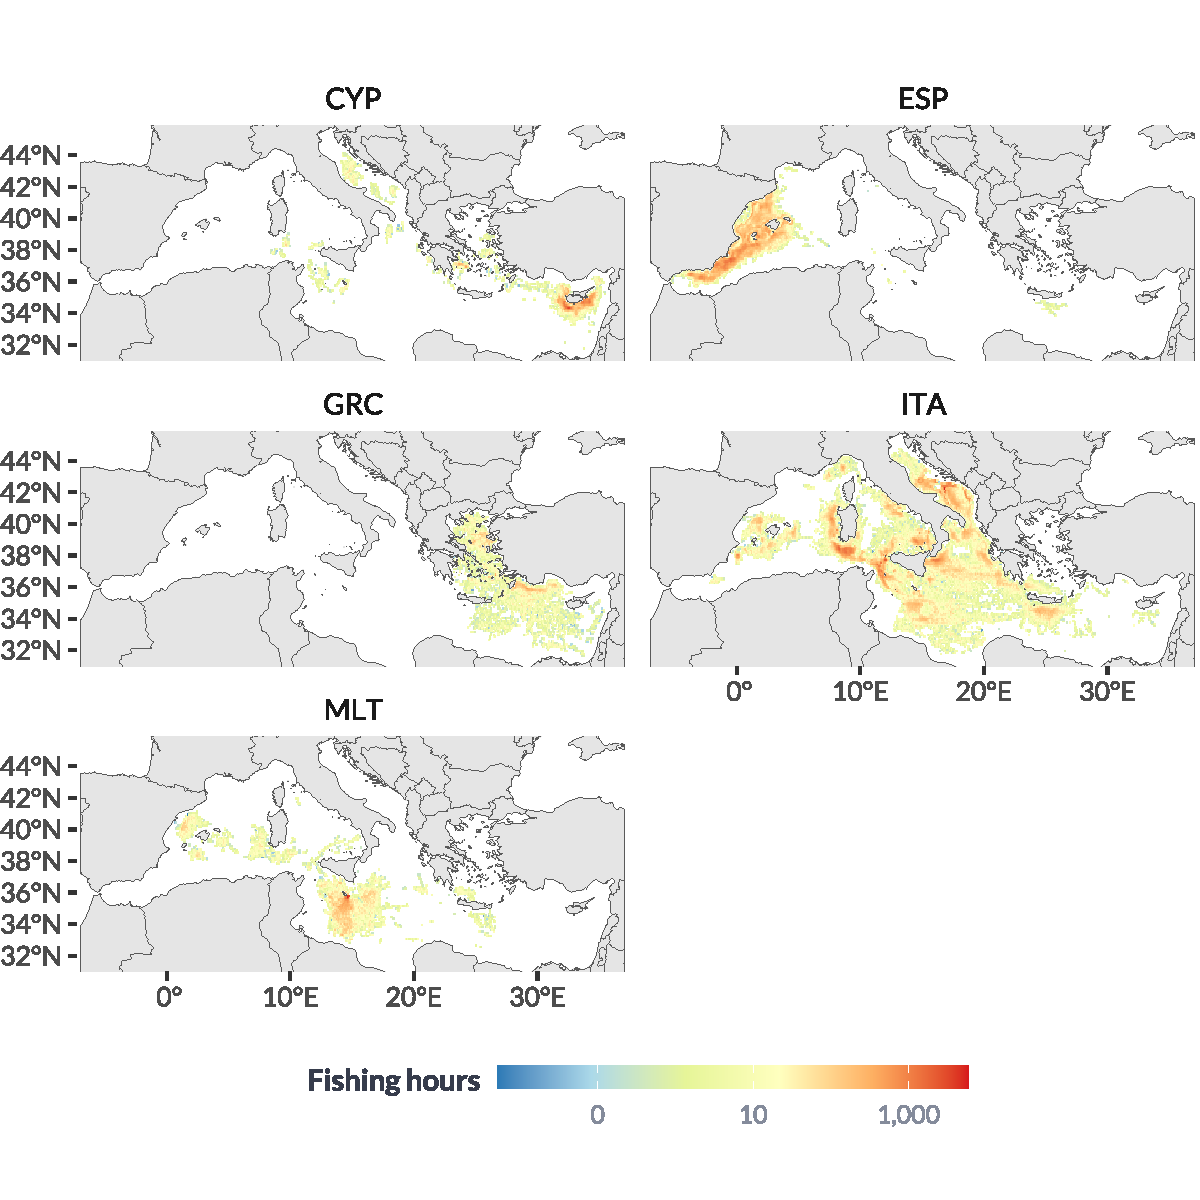
\includegraphics[width=1\linewidth, trim=0 1.2cm 0 1.2cm,clip]{Figures/plots/longline_countries.pdf}
    \caption{Sum of longline fishing hours per flag country (2015-2024). CYP = Cyprus; ESP = Spain, GRC = Greece, ITA = Italy, MLT = Malta}
    \label{fig:longline_effort_countries}
\end{figure}

 \begin{figure}[H]
    \centering
    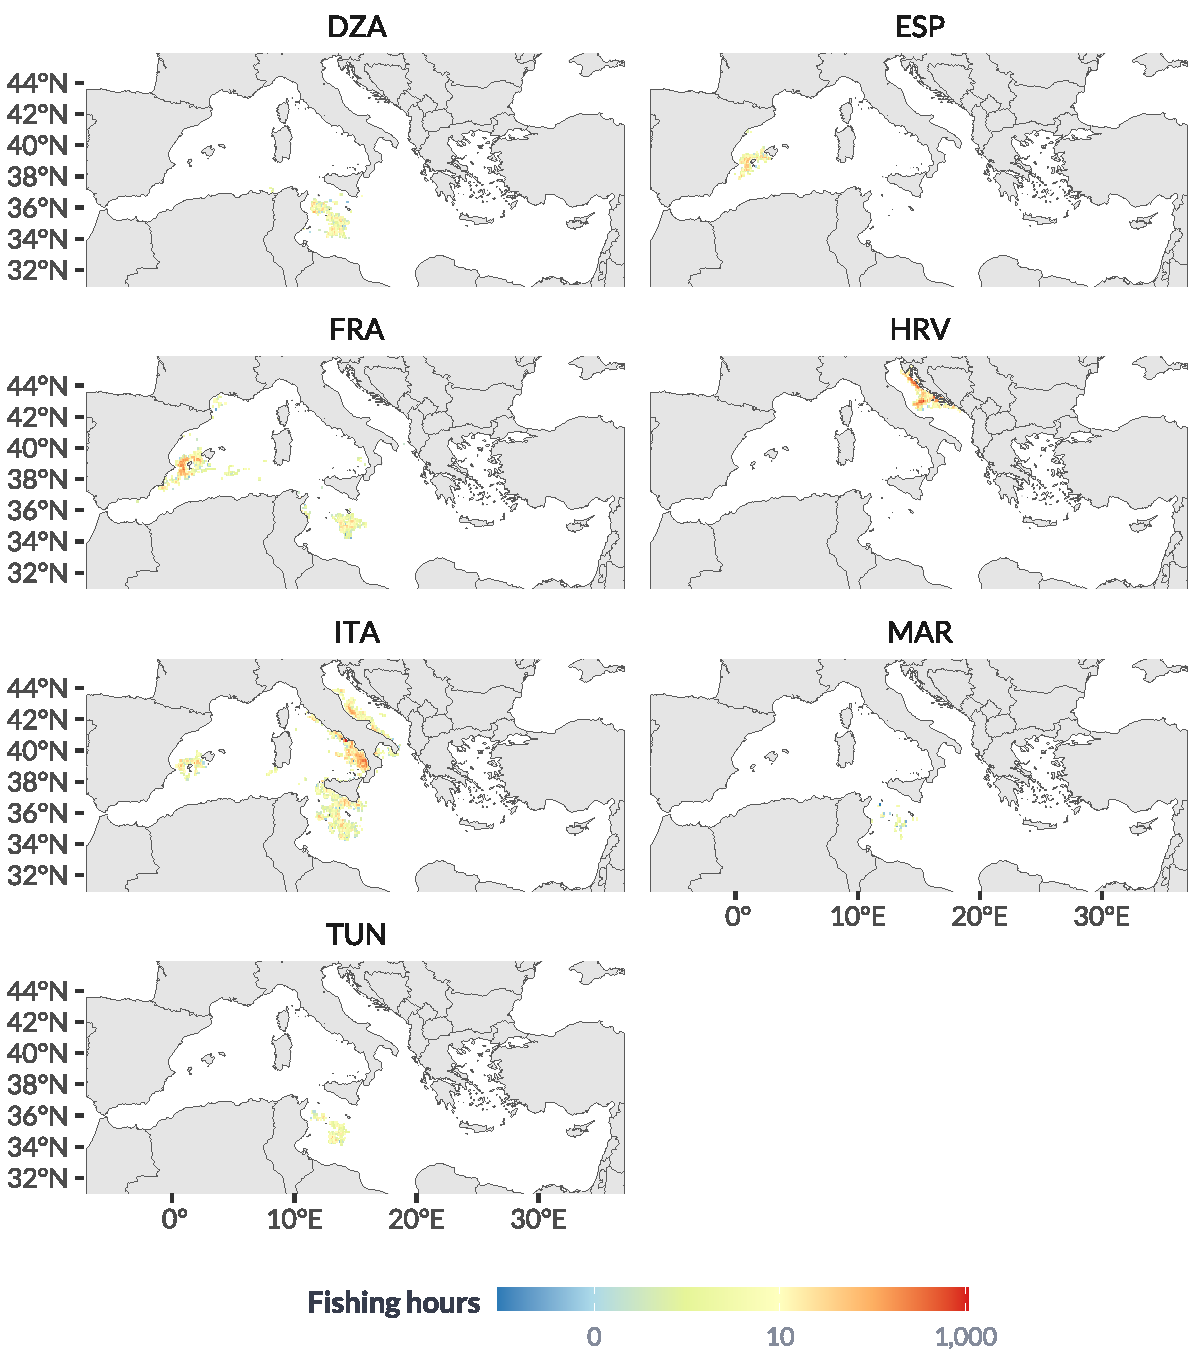
\includegraphics[width=1\linewidth, trim=0 0 0 0,clip]{Figures/plots/seines_countries.pdf}
    \caption{Sum of purse seine fishing hours per flag country (2015-2024). DZA = Algeria, ESP = Spain, FRA = France, 
    HRV = Croatia, ITA = Italy, MAR = Morocco, TUN = Tunisia.}
    \label{fig:seine_effort_countries}
\end{figure}

\end{appendices}

\end{document}